\section{Approach Overview}
\label{overview:sec}

\subsection{Important Concepts}
\label{concepts:sec}

First, we formally define the PDG, multi-version PDG, changed/unchanged statements, and context to conduct our approach's overview. Within these definitions, We re-use the definition of program dependency graph and multi-version program dependency graph from Partachi et al.'s research \cite{flexeme-fse20}.

\begin{Definition}[Program Dependence Graph]
	The \textbf{program dependency graph (PDG)} is a directed graph that contains a node-set $N$ with a set of edges $E$ that represents the relationship among the nodes. The relationship types include data dependency and control dependency.
\end{Definition}

As shown in figure \ref{fig:multi-version-pdg}, the graph with all nodes labeled $i$, and the graph with all nodes labeled with $j$ is the PDG for the version $i$ and version $j$ of the method $FormatYear$. After having these two PDGs, we can define the multi-version program dependency graph.

\begin{Definition}[Multi-version Program Dependence Graph]
	The \textbf{multi-version program dependency graph (Multi-version PDG$^{i,j}$)} is a directed graph that generated from the disjoint union of all nodes and edges between the version $i$ and version $j$.
\end{Definition}

For example, in figure \ref{fig:multi-version-pdg}, the third graph that contains the nodes labeled with $i$, $j$, and $i, j$ is the multi-version PDG$^{i,j}$ combined from the two PDGs for version $i$ and $j$ for the method $FormatYear$. In this graph, the nodes labeled with $i$ or $j$ are the nodes that appeared only in the PDG for version $i$ or $j$. And the nodes labeled with $i, j$ are the nodes that appeared in the PDG for both version $i$ and $j$. With the multi-version PDG$^{i,j}$, we make the definition for the changed/unchanged statements.

\begin{Definition}[Changed/Un-changed Statements]
	The \textbf{changed statements} between version $i$ and $j$ are the statements that are added or deleted to changed the code from version $i$ to version $j$. The modification on an existing statement in version $i$ is regarded as a new statement addition with an old statement deletion. The \textbf{un-changed statements} between version $i$ and $j$ are the statements that keep the same in both version $i$ and version $j$.
\end{Definition}

The figure \ref{fig:multi-version-pdg} can be used an example to show both the changed and un-changed statements between version $i$ and $j$ for the method $FormatYear$. As seen in the multi-version PDG$^[i,j]$ for the method $FormatYear$, the statements $int\, next = i + 1;$ and $var\, next = i + 1;$ that are labeled with $i$ or $j$ are the changed statements between version $i$ and $j$ while the rest statements that are labeled with $i, j$ in the graph are the un-changed statements between version $i$ and $j$.

\begin{Definition}[Context]
	The context of a changed node (changed statement) $n$ is a sub-graph of the multi-version PDG that includes all un-changed nodes (un-changed statements) that are the $k$-hops neighbor of the changed node $n$ with the edges among them.
\end{Definition}

To better understand the context of a changed statement, we still use the figure \ref{fig:multi-version-pdg} as an example to explain. For the statement $int\, next = 1 + 1;$ in the multi-version PDG$^{i,j}$, we select the sub-graph that contains all $k$-hops neighbors as the context. When $k=1$, the sub-graph is built with three statements that labeled with $i, j$ in the multi-version PDG$^{i,j}$.

\begin{figure*}[t]
	\centering
	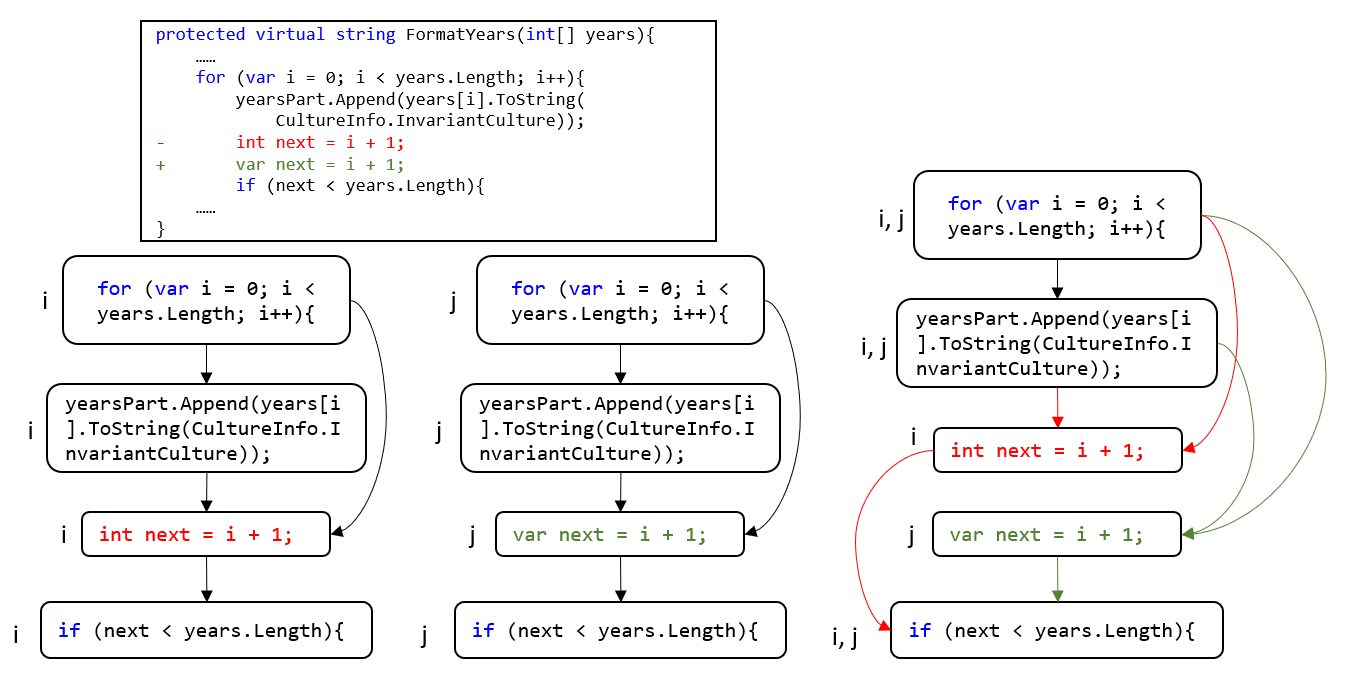
\includegraphics[width=5.3in]{figures/multi-version-graph.png}
	\vspace{-6pt}
	\caption{Multi-Version PDG Example}
	\label{fig:multi-version-pdg}
\end{figure*}

\subsection{Architecture Overview}

After having the definition for the important concepts, we use them to describe the overview of our approach. Within our approach, there are three main steps. We will introduce them one by one.

\subsubsection{Step 1. Building Multi-version Graph and Context}

First, \tool accepts two versions $i$ and $j$ of source code. Following the existing study from Partachi et al. \cite{flexeme-fse20}, \tool firstly generates the PDGs for both the version $i$ and version $j$ for the source code. Next, to construct the multi-version PDG$^{i,j}$, \tool starts from the initial version $i$. \tool uses the PDGs and the Git diff tool on the source files to determine changed and unchanged nodes. Added nodes are introduced to the multi-version PDG$^{i,j}$ as they appear in the newer version $j$. \tool retains nodes deleted across the versions and uses a different label (label $i$) on the nodes to represent the deletion. The unchanged nodes between versions are matched by using string similarity to filter candidates and line-span proximity to rank them. When considering the edge changes, \tool back-propagates the delete nodes to edges flowing into them. Also, \tool considers and adds all unmatched edges in the newer version $j$ to the multi-version PDG$^{i,j}$ as the edges relevant to the added nodes. After having the constructed multi-version PDG$^{i,j}$, for each changed node in the graph, \tool collects all unchanged nodes within the $k$-hops and the edges between them to build a sub-graph as the context for the changed node. The multi-version PDG$^{i,j}$ and the context for each changed node in it will be used as the input for the next step.

\subsubsection{Step 2. Context-aware Graph-based Code Change Clustering Learning Model}

By having the multi-version PDG$^{i,j}$ as the input, \tool firstly uses an advanced GCN model \cite{} that can deal with the nodes with different labels to learn the representation vectors $v_p$ for each node $n_p$ in the graph. For each changed node $n_c$ in $n_p$, \tool collects all unchanged node representation vectors in the context as a matrix. It then uses a fully connected layer to convert it to a vector $v_pc$ to represent all context information for the changed node $n_p$. Next, \tool generates the final representation vector $v'_p$ for changed node $n_p$ by using the cross product between $v_p$ and $v_pc$. With the representation vector $v'_p$ for all changed nodes $n_p$, \tool uses the agglomerative clustering algorithm to cluster the changed nodes into different concerns. Because the number of concerns in the real world commits is not known for \tool, \tool uses a trainable threshold for the linkage when merging the clusters. The output of this step is the clustering results $C$ from the clusters for all changed nodes in the multi-version PDG$^{i,j}$.  

\subsubsection{Step 3. Clustering Updating with the Code Clone}

After having the clustering results $C$ from step 2, in this step, we use the existing state-of-the-art code clone tool \cite{} to detect if there is a code clone between the changed statements $Stmt_m$ and $Stmt_n$ in the multi-version PDG$^{i,j}$. If so, we check the clustering results for $Stmt_m$ and $Stmt_n$ in $C$. If they are clustered to different concerns, \tool updates the clustering results for $Stmt_m$ and $Stmt_n$ to keep them in the same concern based on the code clone results. After going through all changed statements pairs $Stmt_m$ and $Stmt_n$ with this process, \tool has the final clustering results $C'$ for each changed statement between the version $i$ and $j$.

\begin{figure*}[t]
	\centering
 	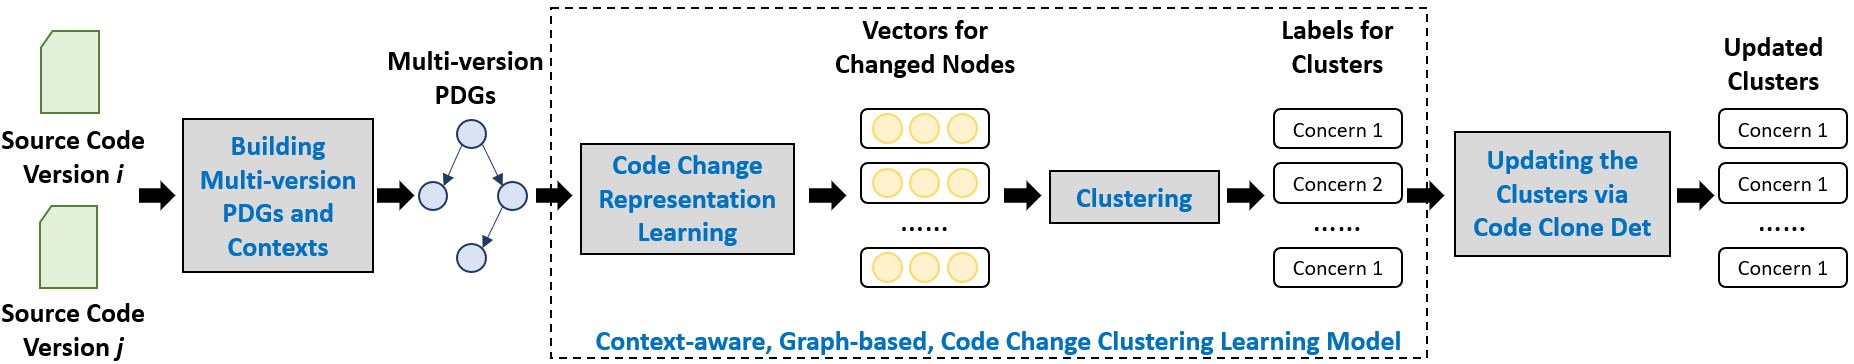
\includegraphics[width=6.5in]{figures/overview.png}
	\vspace{-6pt}
	\caption{Architecture Overview}
	\label{fig:overview}
\end{figure*}

